%%%%%%%%%%%%%%%%%%%%%%%%%%%%%%%%%%%%%%%%%%%%%%%%%%%%%%%%%%%%%%%%%%%
%%%%%%%%%%%%%%%%%%%%%%%%%%%%%%%%%%%%%%%%%%%%%%%%%%%%%%%%%%%%%%%%%%%
%%%%%%%%%%%%%%%%%%%%%%%%%%%%%%%%%%%%%%%%%%%%%%%%%%%%%%%%%%%%%%%%%%%
%%% Potentially useful slides from previous talks 

\begin{frame}{(A Canonical) Classical Planning Language}

{\small

\textbf{Definition.} \emph{A \textblue{planning task} is a 4-tuple
  \textblue{$\Pi=(V,A,I,G)$} where:\vspace{-0.1cm}
\begin{itemize}
\item $V$ is a set of \textblue{state variables}, each $v \in V$ with
  a finite \textblue{domain} $D_v$.\vspace{-0.1cm}
\item $A$ is a set of \textblue{actions}; each $a \in A$ is a triple
  $(\pre_a,\eff_a,\cost_a)$, of \textblue{precondition} and
  \textblue{effect} (partial assignments), and the action's
  \textblue{cost} $\cost_a \in \realnumbers^+_0$.\vspace{-0.1cm}
\item \textblue{Initial state} $I$ (complete assignment),
  \textblue{goal} $G$ (partial assignment).
\end{itemize}}

\textred{\notesym~Solution (``Plan''): Action sequence mapping $I$
  into $s$ s.t.\ $s \models G$.}

\medskip \smallskip \pause

\begin{tabular}{ll}
\hspace{-0.2cm}\begin{minipage}{0.35\textwidth}
\noindent
\textbf{``Logistics'' Example:} 
\end{minipage} &
\begin{minipage}{0.4\textwidth}
\includegraphics[height=2.0cm]{log-ac}
\end{minipage} 
\end{tabular}

\vspace{-0.2cm}

\begin{itemize}
\item \textblue{State variables} $V$: $\mathit{truck}: \{A,B,C,D\}$;
  $\mathit{pack1}: \{A,B,C,D,T\}$.\vspace{-0.15cm}\pause
\item \textblue{Initial state} $I$: $\mathit{truck}=A$,
  $\mathit{pack1}=C$.\vspace{-0.15cm}
\item \textblue{Goal} $G$: $\mathit{truck}=A$,
  $\mathit{pack1}=D$.\vspace{-0.15cm}\pause
\item \textblue{Actions} $A$ (unit costs): $\mathit{drive}(x,y)$,
  $\mathit{load}(p,x)$, $\mathit{unload}(p,x)$. E.g.:
  $\mathit{load}(\mathit{pack1},x)$ precondition $\mathit{truck}=x,
  \mathit{pack1}=x$, effect $\mathit{pack1}=T$.
\end{itemize}

%% \begin{itemize}
%% \item $V = \{t, p_1, \dots, p_5\}$ with $D_c = \{V, E, T, M\}$ and
%%   $D_{p_i} = \{V, E, T, M, t\}$.\vspace{-0.1cm}\pause
%% \item $A = \{\mathit{load}(i,x), \mathit{drop}(i,x),
%%   \mathit{move}(x,x')\}$ where, \eg,
%%   $\textred{\pre_{\mathit{load}(i,x)} = \{(t,x), (p_i,x)\}}$ and
%%   $\textred{\eff_{\mathit{load}(i,x)} =
%%     \{(p_i,t)\}}$.\vspace{-0.1cm}\pause
%% \item $I = \{(t,V), (p_1,\mathit{V}), \dots\}$. $G =
%%   \{(p_1,\mathit{T}), \dots\}$.
%% \end{itemize}

}

\end{frame}


% TALK: ``To convince you that this is not limited to talking about
% trucks and packages ...''. Be very brief on these 2 slides.
%
\begin{frame}{Semantic BPM@SAP \hfill \scriptsize [\cite{hoffmann:etal:jair-12}]}

{\small

\vspace{-0.5cm}

\begin{center}
\begin{tabular}{cc}
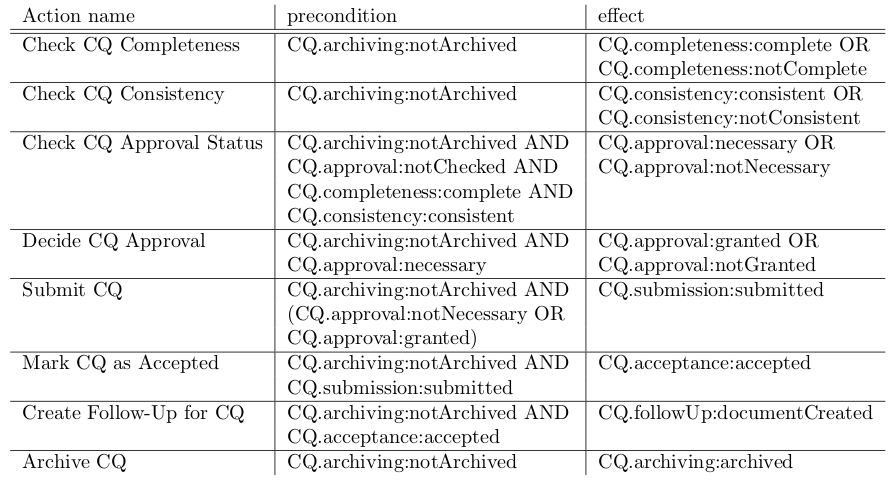
\includegraphics[height=4.0cm]{sam} \hspace{0.2cm} & 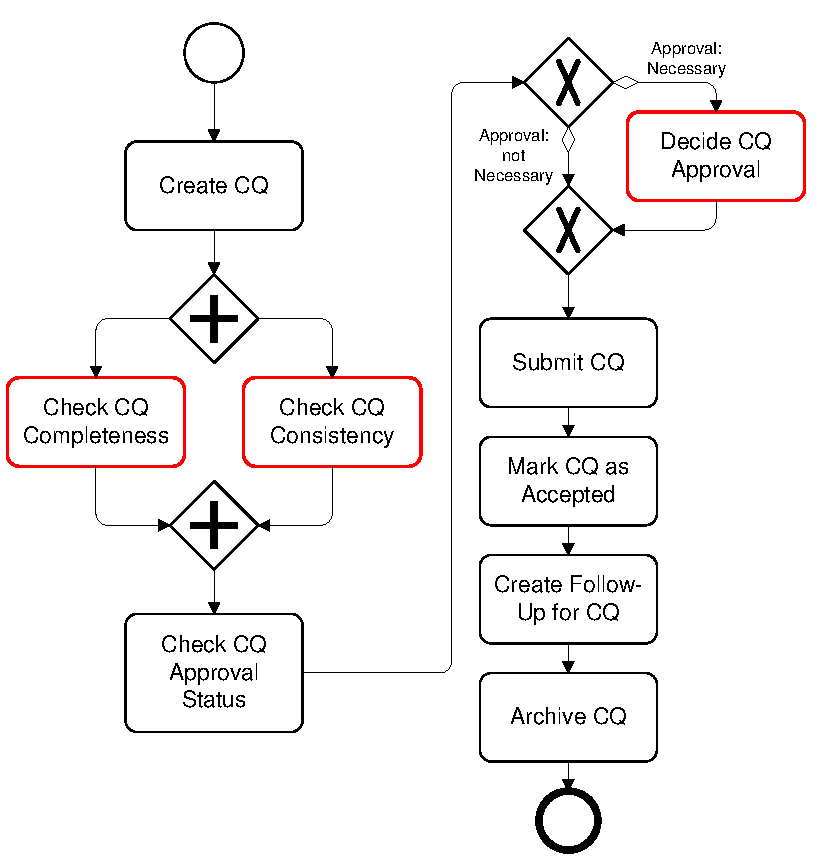
\includegraphics[height=4.0cm]{process} 
\end{tabular}
\end{center}

\vspace{-0.2cm}

\begin{itemize}
\item \textbf{Planning model:} SAP-scale model of activities on
  Business Objects; desired process endpoint.
\item \textbf{Solution:} Process template leading to this point.
\item \textbf{Key advantage:} \textred{Eases process
  creation. Automation wrpto activities/objects (\ie, arbitrary models
  thereof).}
\end{itemize}

}

\medskip

\end{frame}


\begin{frame}{Controlling Modular Printers@Xerox \hfill \scriptsize [\cite{ruml:etal:jair-11}]}

{\small

\vspace{-0.4cm}

\begin{center}
\begin{tabular}{cc}
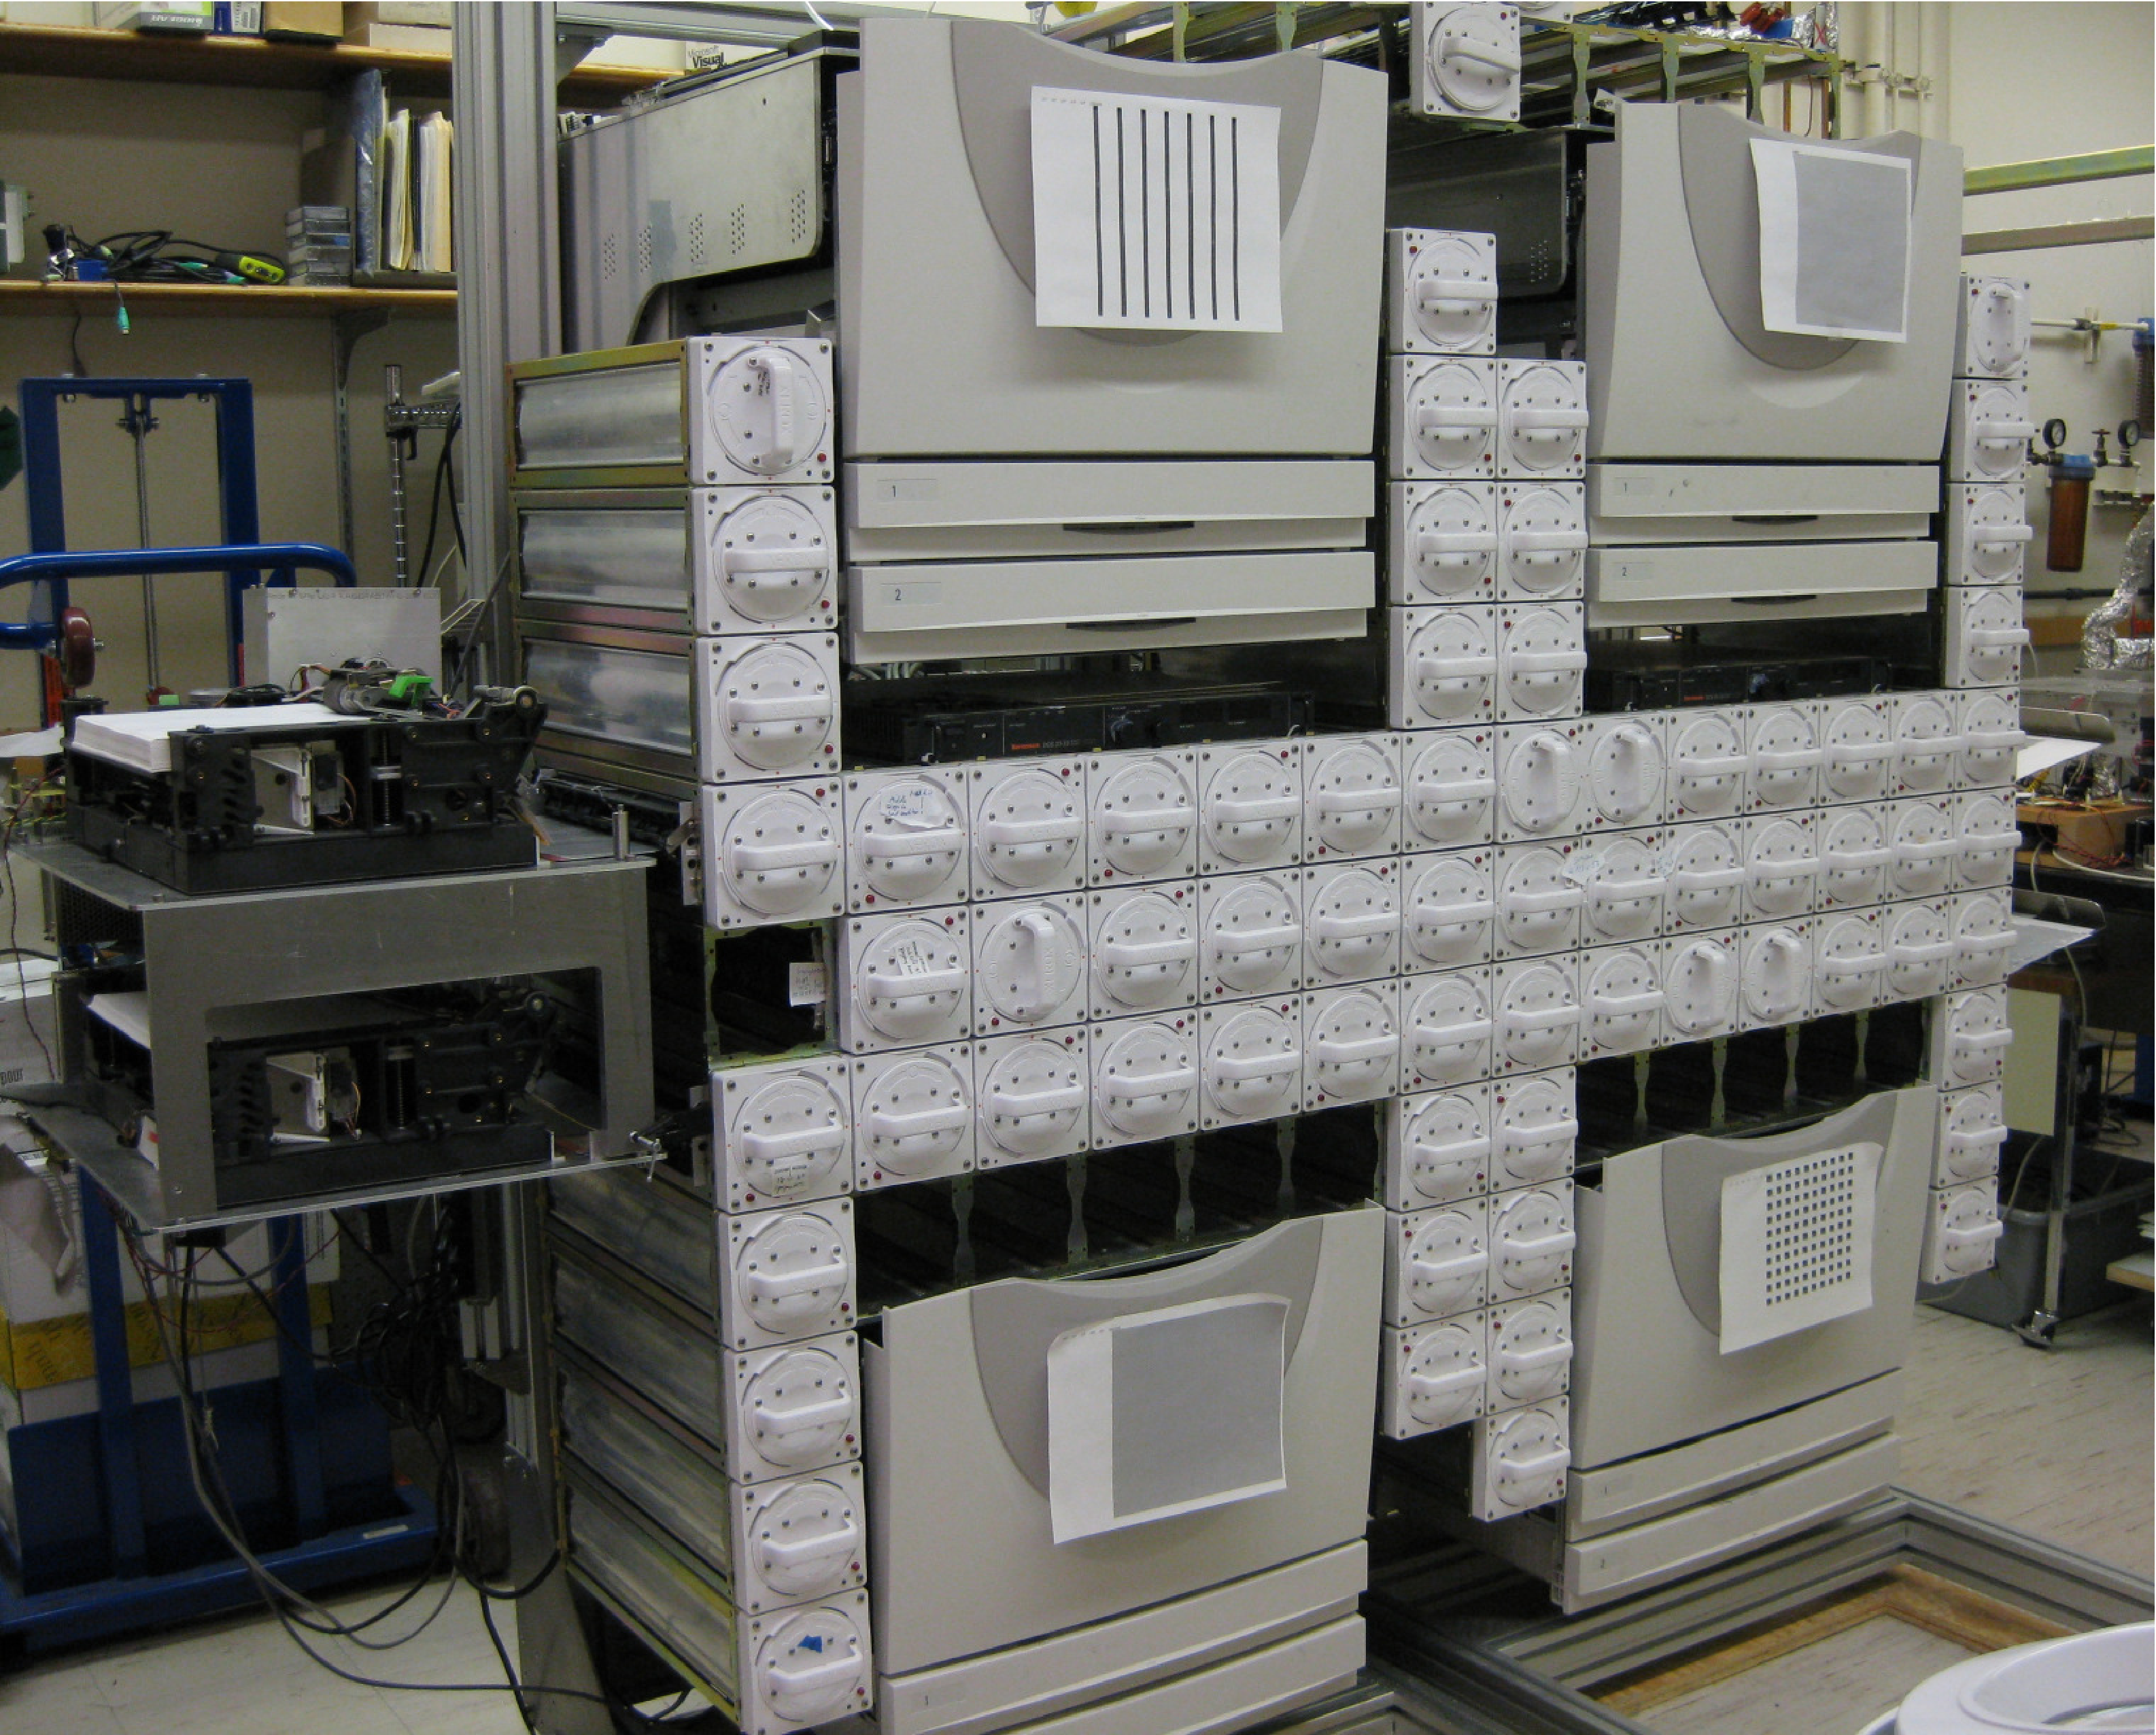
\includegraphics[height=3.7cm]{wheeler-fixture-photo-2} &
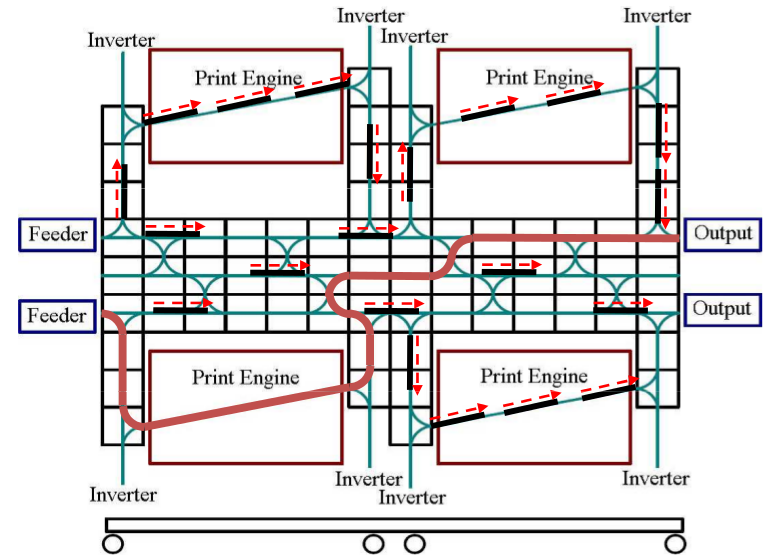
\includegraphics[height=4cm]{wheeler-fixture-paperpaths} 
\end{tabular}
\end{center}

\vspace{-0.1cm}

\begin{itemize}
\item \textbf{Planning model:} Modular printer components, printer
  configuration, current jobs.
\item \textbf{Solution:} Optimal schedule of current jobs.
\item \textbf{Key advantage:} \textred{Automation wrpto possible
  configurations: A controller for a system whose exact design is not
  known at software-design time.}
\end{itemize}

}

\medskip

\end{frame}


\begin{frame}{Model-Based (aka Automated) Planning@Robotics: Why?}

\noprehandout{

\medskip

{\small

{\centering

\begin{tabular}{ccc}
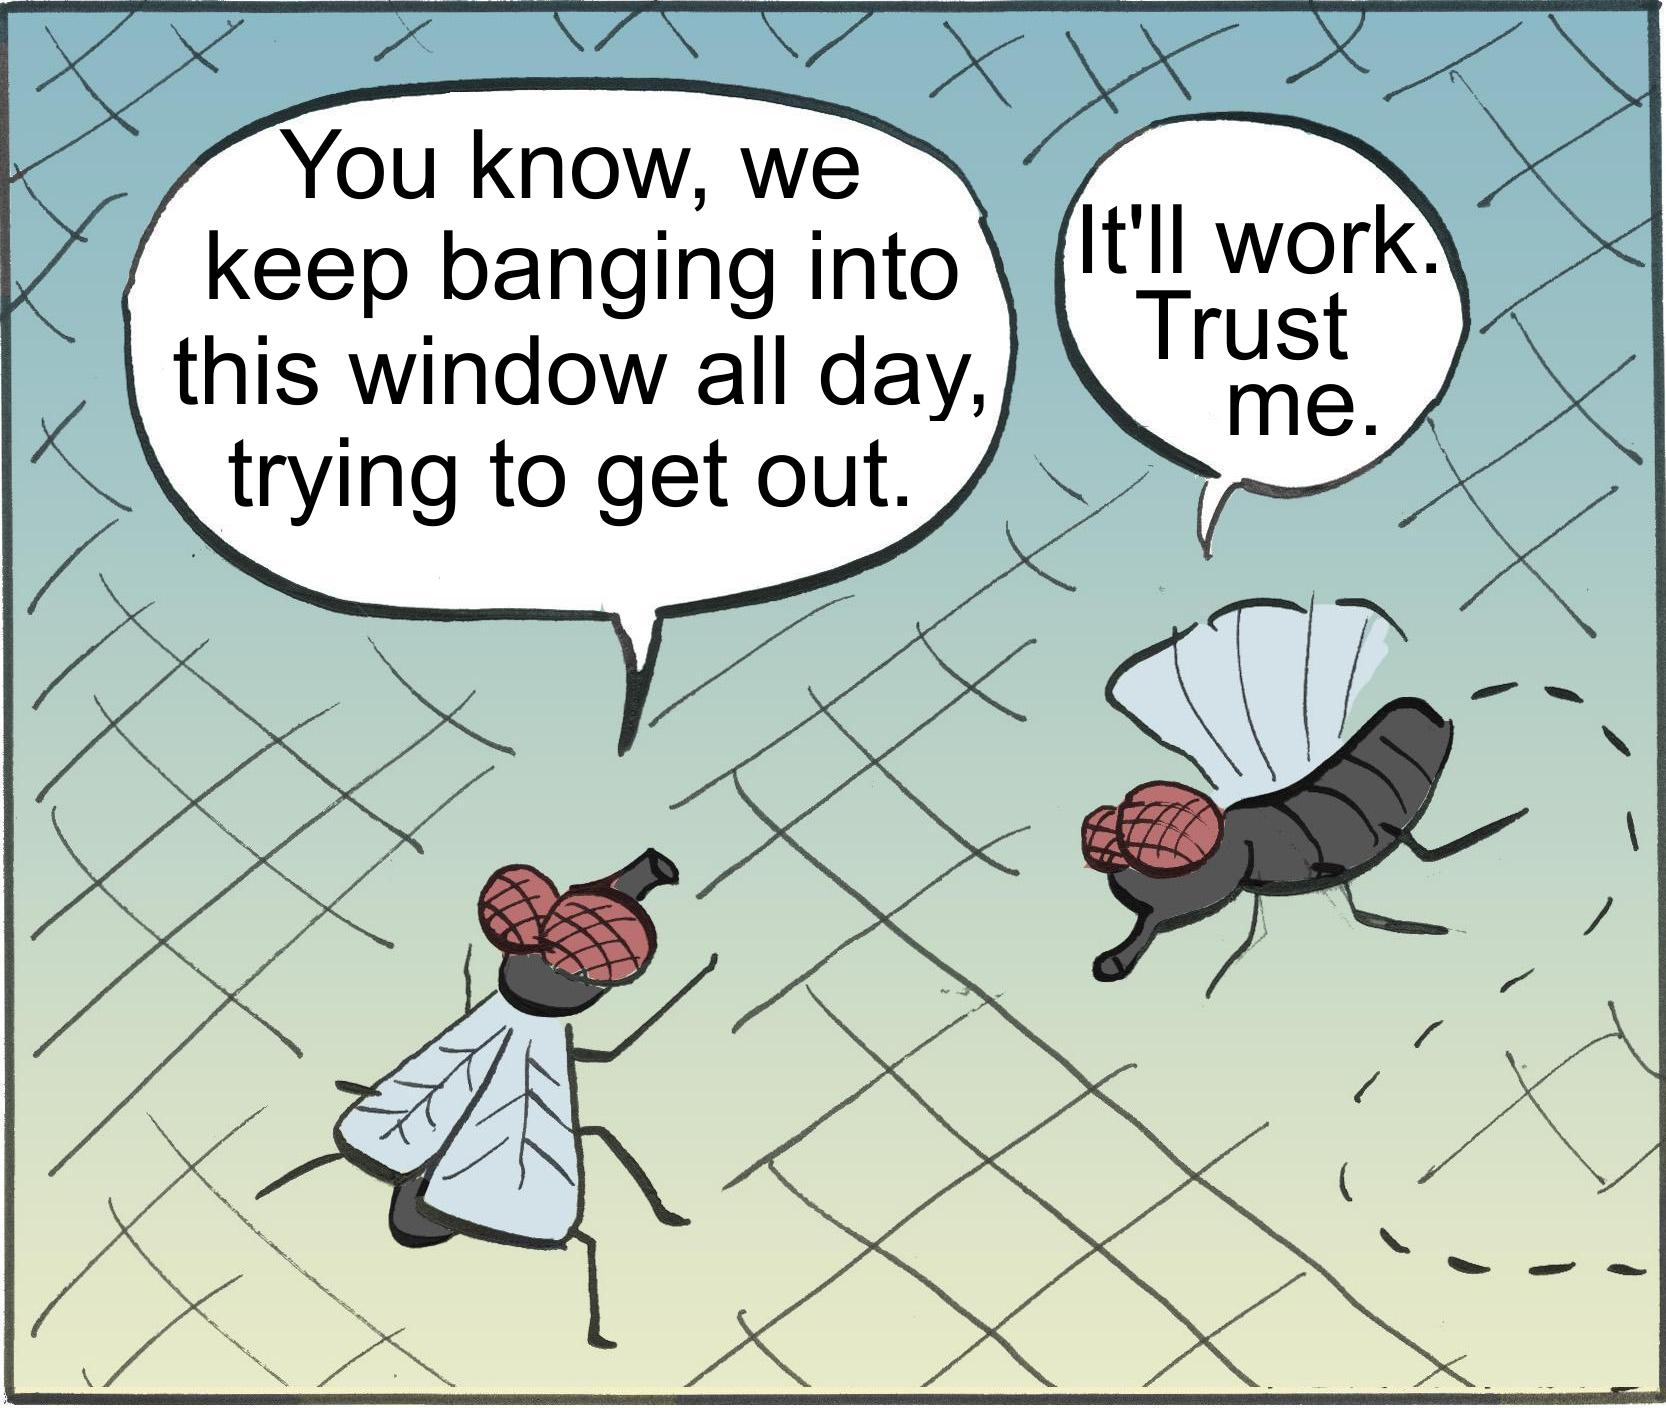
\includegraphics[height=3.5cm]{flies-window.jpg} & \pause

\includegraphics[height=3.5cm]{flies-vs.jpg} & 
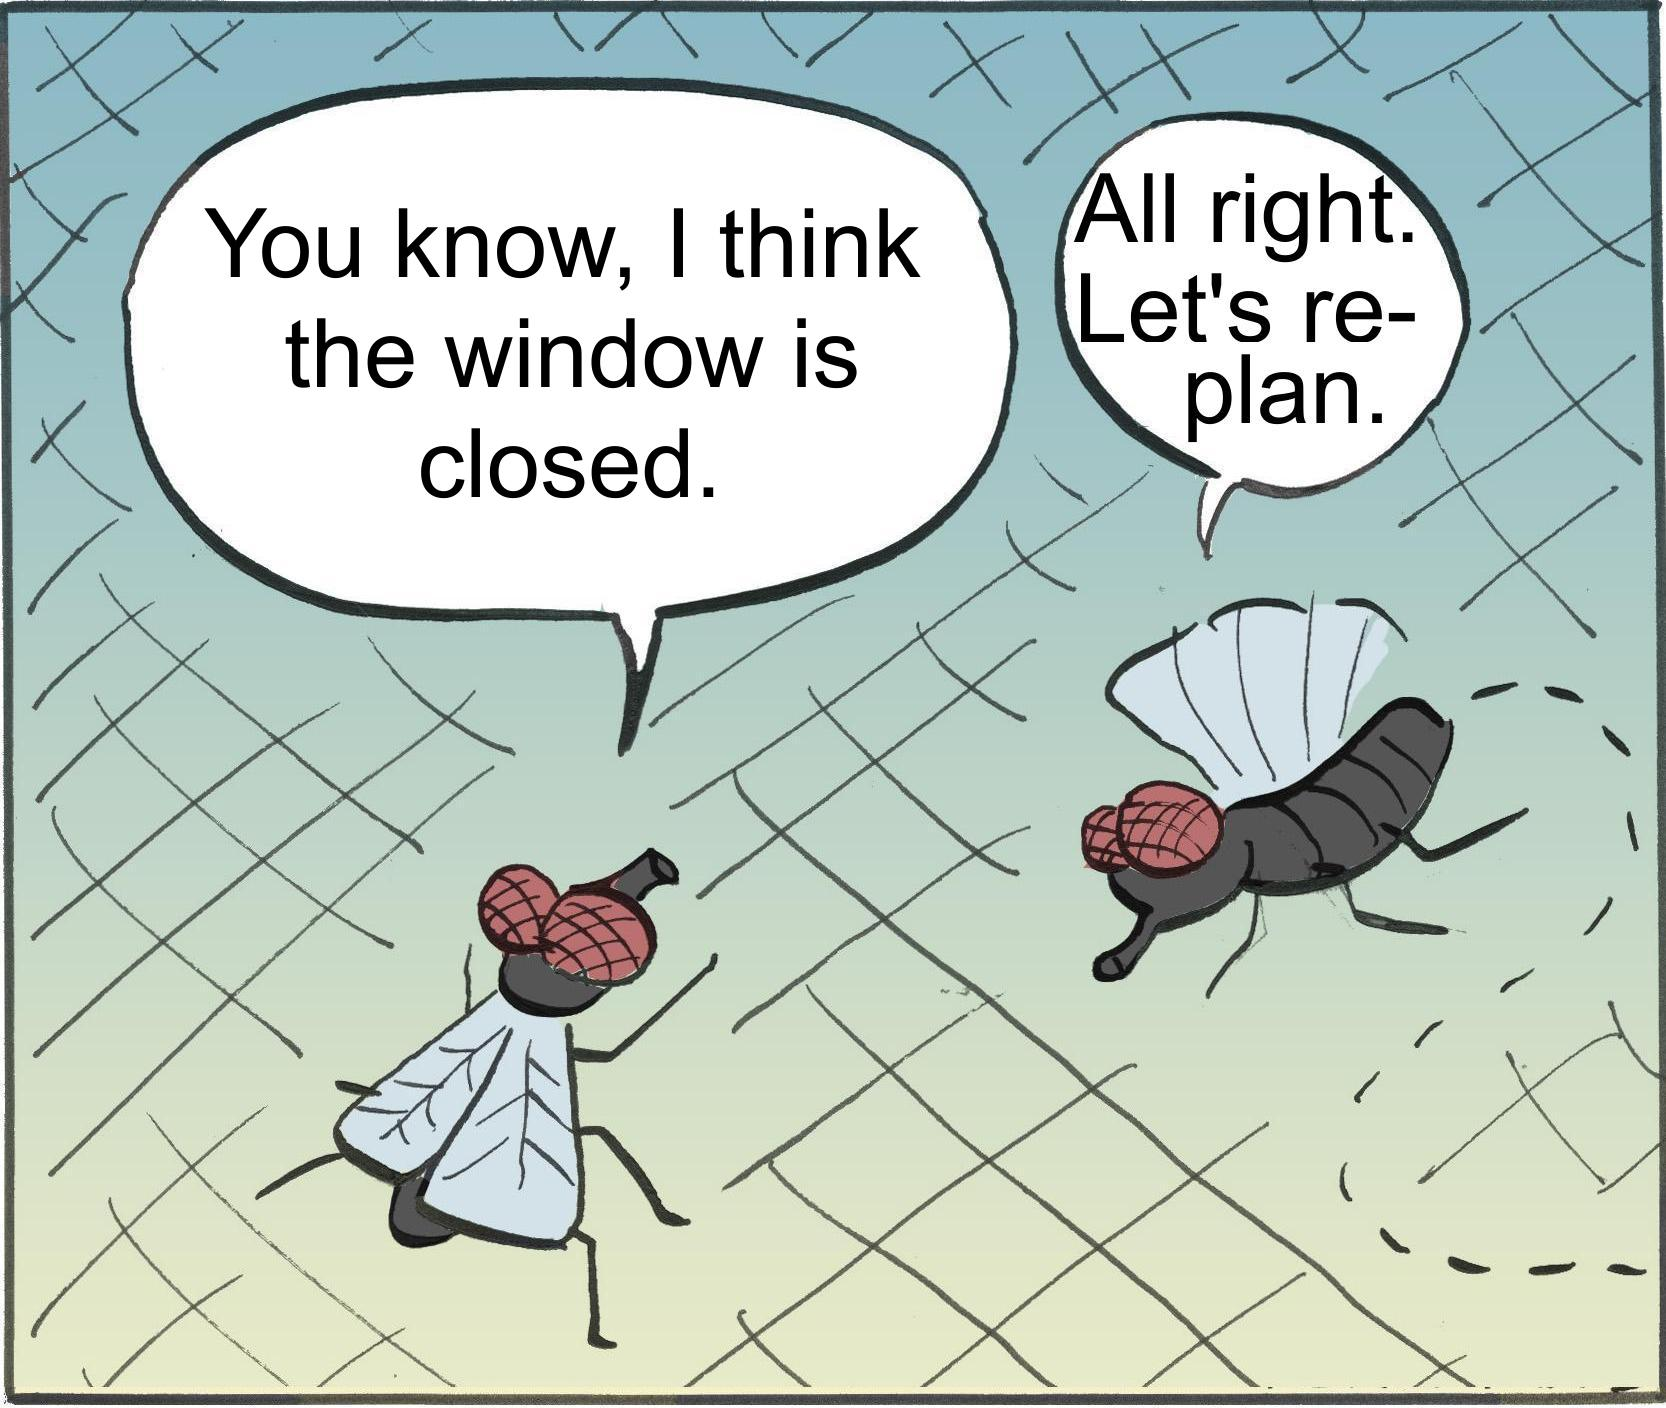
\includegraphics[height=3.5cm]{flies-window-planning.jpg} 
\end{tabular}

}

\medskip \medskip \pause

% TALK: Now, for navigation and dynamic obstacles of course
% flexibility is standard and does not require full-scale high-level
% planning. But think about more complex domains, like semi-automated
% production, aerial vehicle scheduling and control, underwater
% vehicles, supply chains, and even street traffic if unexpected
% events include eg unexpected behavior by other traffic participants.
%
\textbf{Plan-Based Control:}

\vspace{-0.1cm}

\begin{itemize}
\item Planning model allows to capture arbitrary states, actions,
  goals.
\item Reacting to arbitrary state/goal change (within fixed model):
  \textblue{Re-planning}.
\item Explicit model/plan allows robot to \textblue{reason about
  plan/what went wrong}, instead of just following a prescribed
  recipe/workflow.
\end{itemize}

\textred{\notesym~Long-term autonomy; dynamic environments (unexpected
  events).}

}

\medskip

}

\end{frame}


\begin{frame}{Planning Framework Dimensions (\& Classical Planning)}

\noprehandout{

\medskip

{\small

{\centering

\begin{tabular}{ccc}
\visible<7-|handout:1>{
\textblue{\textbf{You GET (classical planning)}} & \textbf{vs.} & \textred{\textbf{You NEED (robotics)}}\\\hline\hline
}
\textblue{discrete} & vs.\ & \textred{continuous}\\\hline
\visible<2-|handout:1>{
\textblue{instantaneous actions} & vs.\ & \textred{temporal actions}\\\hline
}
\visible<3-|handout:1>{
\textblue{sequential plans} & vs.\ & \textred{concurrent plans}\\\hline
}
\visible<4-|handout:1>{
\textblue{fully observable} & vs.\ & \textred{partially observable}\\\hline
}
\visible<5-|handout:1>{
\textblue{deterministic} & vs.\ & \textred{non-deterministic/stochastic}\\\hline
}
\visible<6-|handout:1>{
\textblue{goal-state condition} & vs.\ & \textred{temporal goals/preferences/rewards}
}
\end{tabular}

}

\bigskip

\visible<8-|handout:1>{
\textbf{So why bother?}
}

\vspace{-0.1cm}

\visible<9-|handout:1>{
\begin{itemize}
\item \textblue{Fast re-planning}. (Classical planning already is
  \textbf{PSPACE}-complete, never mind the more accurate
  variants.)\vspace{-0.1cm}
\item \textblue{``Your need'' actually depends on your system
  architecture}/what the ``Activity Planning'' component is being used
  for.\vspace{-0.1cm}
\item \textblue{Transfer of algorithmic ideas} to richer planning
  problems.
\end{itemize}
}

\vspace{-0.1cm}

\visible<10-|handout:1>{

\textred{\notesym~Classical planning is very restricted, but provides fast mechanisms for
  flexible reactive high-level planning. (And is a good frame for
  basic algorithms research.)}

}

}

\medskip

}

\end{frame}


\begin{frame}{A Successful Family of Solvers: Heuristic Search}

\begin{center}
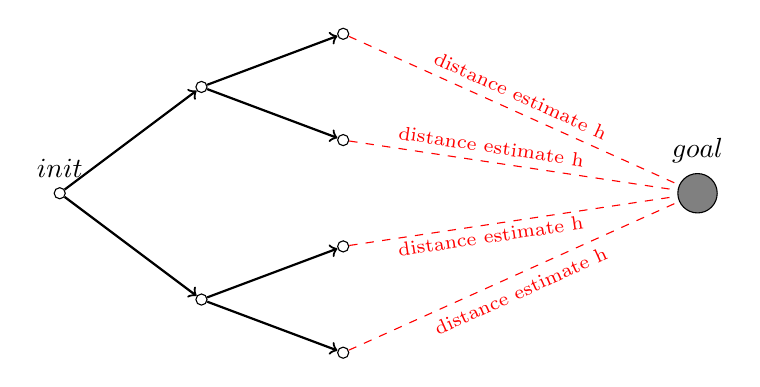
\begin{tikzpicture}[scale=.9]
  \node[circle, draw, fill=gray, minimum height=5mm,
label=above:$\textblue{\text{goal}}$] (Goal) at (9,0) {}; 
  \node[circle,draw, inner sep=0.5mm,
label=above:$\textblue{\text{init}}$] (N0) at (0,0) {};
  \node[circle,draw, inner sep=0.5mm] (N00) at (2,-1.5) {};
  \node[circle,draw, inner sep=0.5mm] (N01) at (2,1.5) {};
  \node[circle,draw, inner sep=0.5mm] (N000) at (4,-2.25) {};
  \node[circle,draw, inner sep=0.5mm] (N001) at (4,-0.75) {};
  \node[circle,draw, inner sep=0.5mm] (N010) at (4,0.75) {};
  \node[circle,draw, inner sep=0.5mm] (N011) at (4,2.25) {};

  \draw[->, thick] (N0) -- (N00);
  \draw[->, thick] (N0) -- (N01);
  \draw[->, thick] (N00) -- (N000);
  \draw[->, thick] (N00) -- (N001);
  \draw[->, thick] (N01) -- (N010);
  \draw[->, thick] (N01) -- (N011);
  
  \draw[dashed, red] (N000) -- node[below,sloped] {
\scriptsize distance estimate h} (Goal);
  \draw[dashed, red] (N001) -- node[below=0.15cm,sloped,left=-1.0cm] {
\scriptsize distance estimate h} (Goal);
  \draw[dashed, red] (N010) -- node[above=0.2cm,sloped,left=-1.0cm] {
\scriptsize distance estimate h} (Goal);
  \draw[dashed, red] (N011) -- node[above,sloped] {
\scriptsize distance estimate h} (Goal);
\end{tikzpicture}
\end{center}

\smallskip

\noteblk{\notesym~Forward state space search. Heuristic function $h$
  maps states $s$ to an estimate $h(s)$ of goal distance.}

\end{frame}


\begin{frame}{Heuristic Functions}

\noprehandout{

\only<1|handout:1>{

\begin{center}
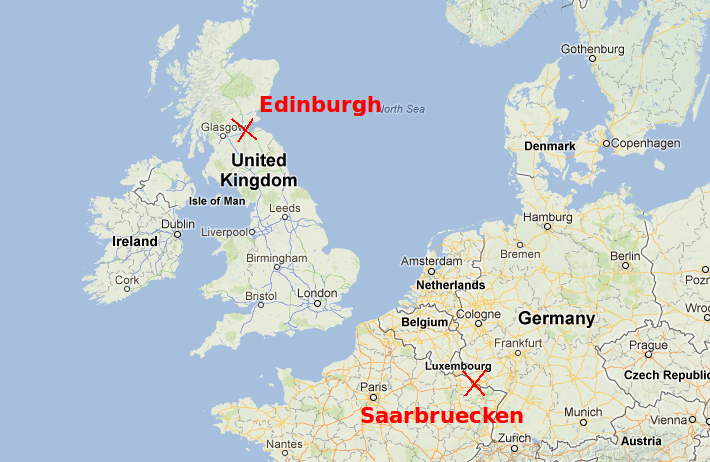
\includegraphics[height=6cm]{europe-map}

\smallskip

\textred{Problem: Find a route from Saarbruecken To Edinburgh.}
\end{center}

\medskip

}
%
\only<2|handout:2>{

\begin{center}
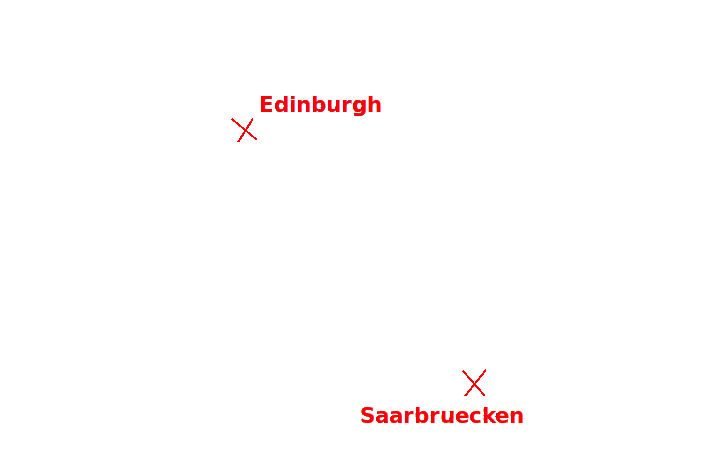
\includegraphics[height=6cm]{europe-nomap}

\smallskip

\textred{Relaxed Problem: Throw away the map.}
\end{center}

\medskip

}
%
\only<3|handout:3>{

\begin{center}
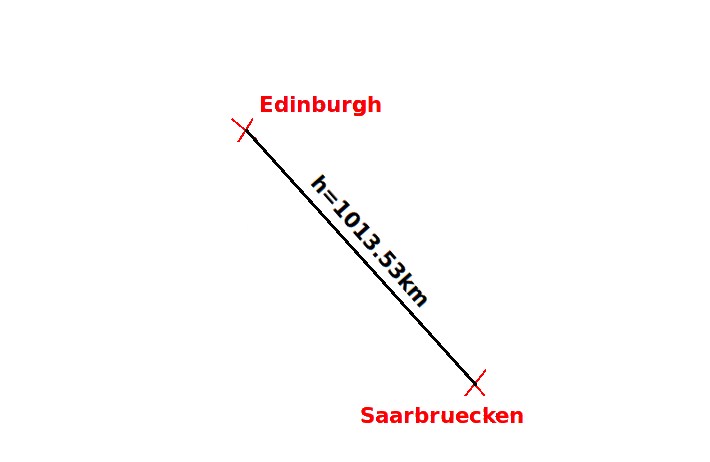
\includegraphics[height=6cm]{europe-nomap-line}

\smallskip

\textred{Heuristic function: Straight line distance.}
\end{center}

\medskip

}
%
% TALK: But HOW to automatically design the ``Simplified Problem'' in
% planning, and how to compute h?

}

\end{frame}


\begin{frame}{Explanation}

{\small

\medskip

{\centering

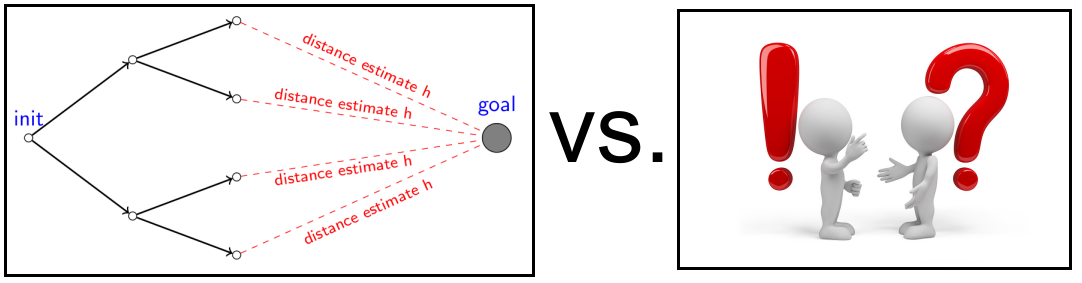
\includegraphics[width=0.8\textwidth]{hsearch-vs-explanation.png} 

\smallskip

\textred{\notesym~If you want to interact with people, you need 
to be able to explain yourself.}

}

\smallskip \pause

{\footnotesize

\begin{itemize}
\item E.g.\ ``\textred{what} I am about to do'', to human co-worker 
in production environment.
\item E.g.\ ``\textred{why} I am doing A and not B'', to human 
supervisor in production environment.\pause
\item So far: ``what'' in terms of inner workings of the chosen plan 
{\scriptsize
[\eg\ \cite{mcguiness:etal:flairs-07,khan:etal:icaps-09,seegebarth:etal:icaps-12}]};
``excuses'' explaining why a plan does not exist (minimal
modifications that would make the task solvable) {\scriptsize
[\eg\ \cite{goebelbecker:etal:icaps-10}]}.
\end{itemize}

\pause

\textred{\notesym~What about explaining the plan decision itself, 
``why this plan''? E.g.\ for simplicity, given state $s$ and
applicable actions $A$ vs.\ $B$, why $A$ and not $B$?}
%
% TALK: Same as last time, though in the meantime I've written a
% project proposal on this last bit ... (it's what you do at my age:
% you don't go ahead and write a paper, instead you write a project
% proposal, so you can hire somebody who will write the paper ...)

}

}

\medskip

\end{frame}


\begin{frame}{Deep Learning}

{\small

\medskip

{\centering

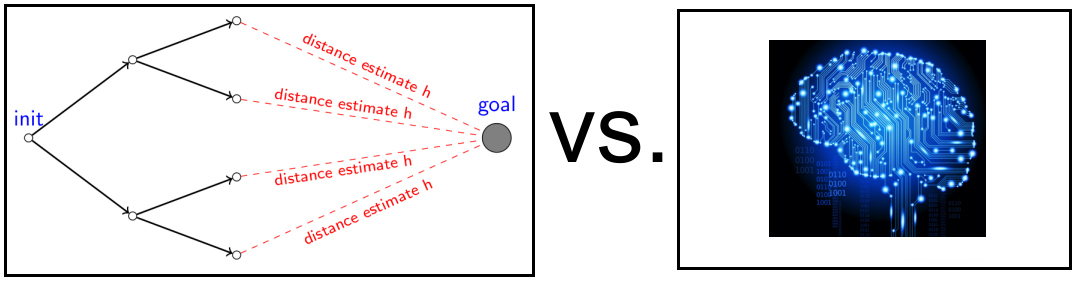
\includegraphics[width=0.8\textwidth]{hsearch-vs-deeplearning.png} 

}

\medskip \pause

\textbf{This can go both ways:}

\begin{itemize}
\item \textred{Using DNN in planning:} design effective planning algorithms, 
satisfy real-time conditions.
\item \textred{Using planning to reign in DNN:} model-based simulation \& analysis of 
future developments.
\end{itemize}

\pause

\textred{\notesym~Safegarding online NN decisions (similar to
AlphaGo/Zero)?}

\medskip 

\textred{\notesym~Model-based simulation for offline validation,
debugging, analysis, testing?}

}

\bigskip

\end{frame}



